% --------------------------------------------------------------
% This is all preamble stuff that you don't have to worry about.
% Head down to where it says "Start here"
% --------------------------------------------------------------
 
\documentclass[12pt]{article}
 
\usepackage[margin=1in]{geometry} 
\usepackage{amsmath,amsthm,amssymb}
 
\newcommand{\N}{\mathbb{N}}
\newcommand{\Z}{\mathbb{Z}}
 
\newenvironment{theorem}[2][Theorem]{\begin{trivlist}
\item[\hskip \labelsep {\bfseries #1}\hskip \labelsep {\bfseries #2.}]}{\end{trivlist}}

\newenvironment{lemma}[2][Lemma]{\begin{trivlist}
\item[\hskip \labelsep {\bfseries #1}\hskip \labelsep {\bfseries #2.}]}{\end{trivlist}}

\newenvironment{exercise}[2][Exercise]{\begin{trivlist}
\item[\hskip \labelsep {\bfseries #1}\hskip \labelsep {\bfseries #2.}]}{\end{trivlist}}

\newenvironment{problem}[2][Problem]{\begin{trivlist}
\item[\hskip \labelsep {\bfseries #1}\hskip \labelsep {\bfseries #2}]}{\end{trivlist}}

\newenvironment{intro}[2][Introduction]{\begin{trivlist}
\item[\hskip \labelsep {\bfseries #1}\hskip \labelsep {\bfseries #2}]}{\end{trivlist}}

\newenvironment{question}[2][Question]{\begin{trivlist}
\item[\hskip \labelsep {\bfseries #1}\hskip \labelsep {\bfseries #2.}]}{\end{trivlist}}

\newenvironment{corollary}[2][Corollary]{\begin{trivlist}
\item[\hskip \labelsep {\bfseries #1}\hskip \labelsep {\bfseries #2.}]}{\end{trivlist}}

\usepackage{graphicx}
\graphicspath{{./}}

\begin{document}
 
% --------------------------------------------------------------
%                         Start here
% --------------------------------------------------------------
 
\title{Project 1}%replace X with the appropriate number
\author{Yunzhong He\\ %replace with your name
204010749} %if necessary, replace with your course title
 
\maketitle

\begin{problem}{1. High Kurtosis and Scale Invariance}
\item{}
For this problem we applied gradient filter to a natural scene image, and plotted the histogram of the gradients at each pixel. Then we fitted the histogram with a generalized Gaussian distribution, and compared it with a regular Gaussian distribution. Lastly, we down sampled the image and applied the same procedure, and compared the results with the original image.\\
\item{1.1 Histogram of convolved image\\}
After applying the gradient filter, we obtained the following histogram.
\begin{center}
		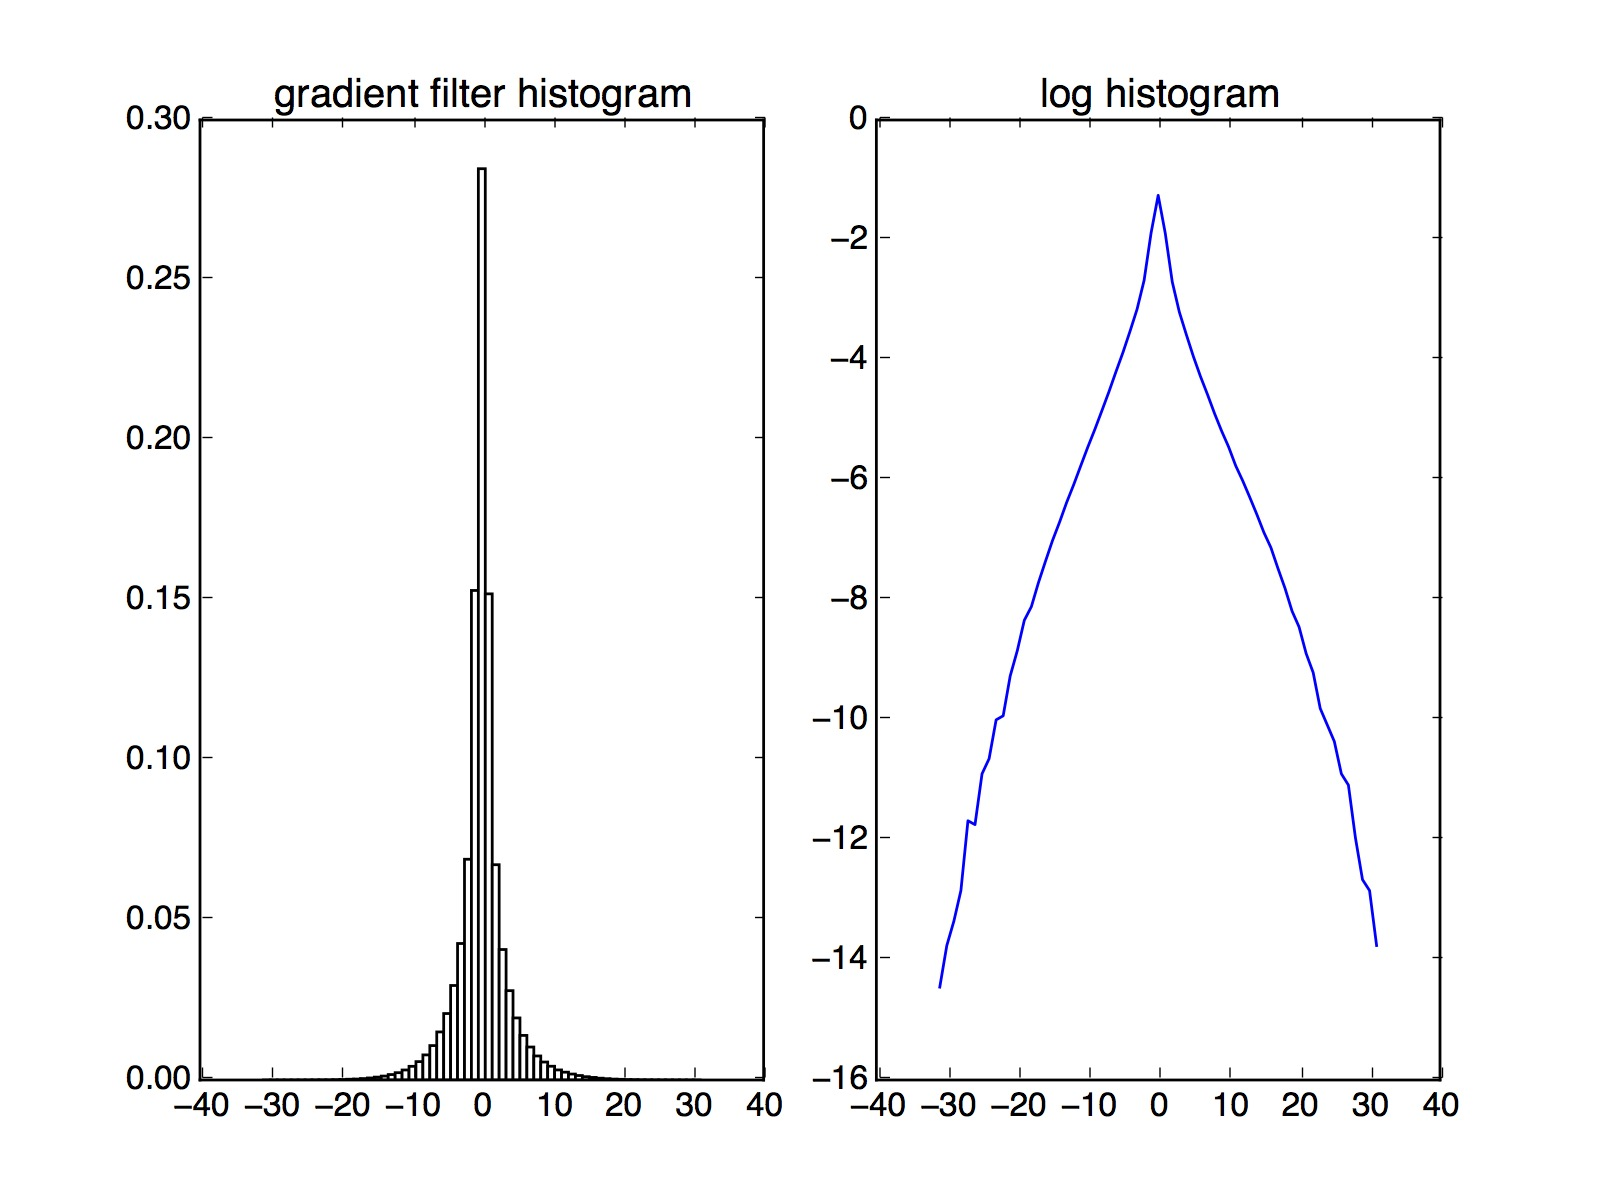
\includegraphics[height=10cm]{results/q1_1.jpg}{\\figure 1 histogram of convolved image}
\end{center}
From the figure 1 above we can see that the histogram is pretty spiky, indicating that the original pixels may not be sampled randomly.\\
\item{1.2 The mean, variance, kurtosis of the histogram is below.}
\begin{center}
\begin{tabular}{l | r}
	mean & -0.0155\\
	variance & 12.72\\
	kurtosis & 5.626\\
\end{tabular}
\end{center}
And we can see that the high kurtosis confirms with the spiky looking of the histogram.\\
\item{1.3} We further fit the histogram with a generalized Gaussian distribution given by
\begin{align*}
	p(x) = \frac{\gamma}{2\sigma\Gamma(1/\gamma)} exp(-(|x-\mu|/\sigma)^{\gamma})
\end{align*}
with the mean and standard deviation we obtaind from 1.2, and obtaind the follwing curve.
\begin{center}
		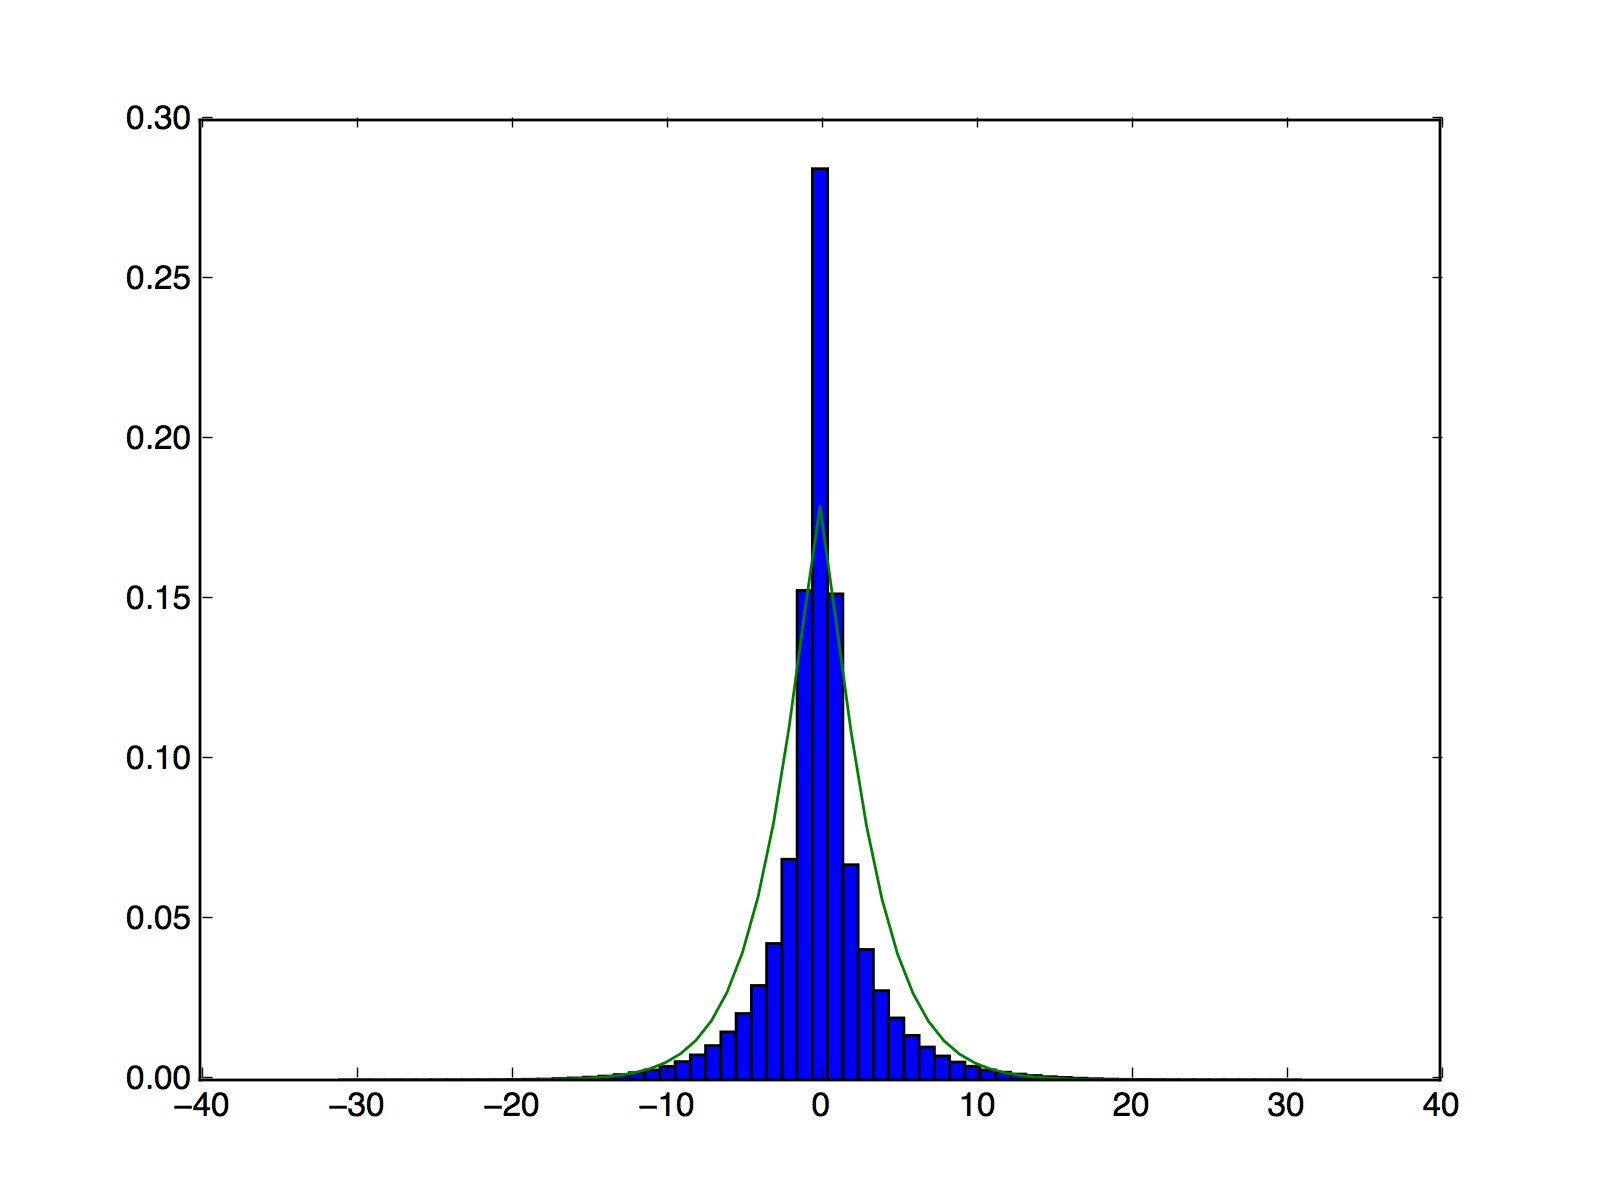
\includegraphics[height=10cm]{results/q1_3.jpg}{\\figure 2 generalized Gaussian fit}
\end{center}
We found the best fit parameter to be $\gamma$ = \textbf{1.22}. Since $\gamma < 2$ we can conclude that the histogram does not follow a Gaussian distribution, meaning the pixels from a natural image are not sampled randomly. Moreover, the high kurtosis, or the $\gamma$ value we found indicates that there must be some structue behind the pixel's distribution.\\
\item{1.4}
For comparision, we also computed a Gaussian using the mean and variance from 1.2, and obtained the following curves.
\begin{center}
		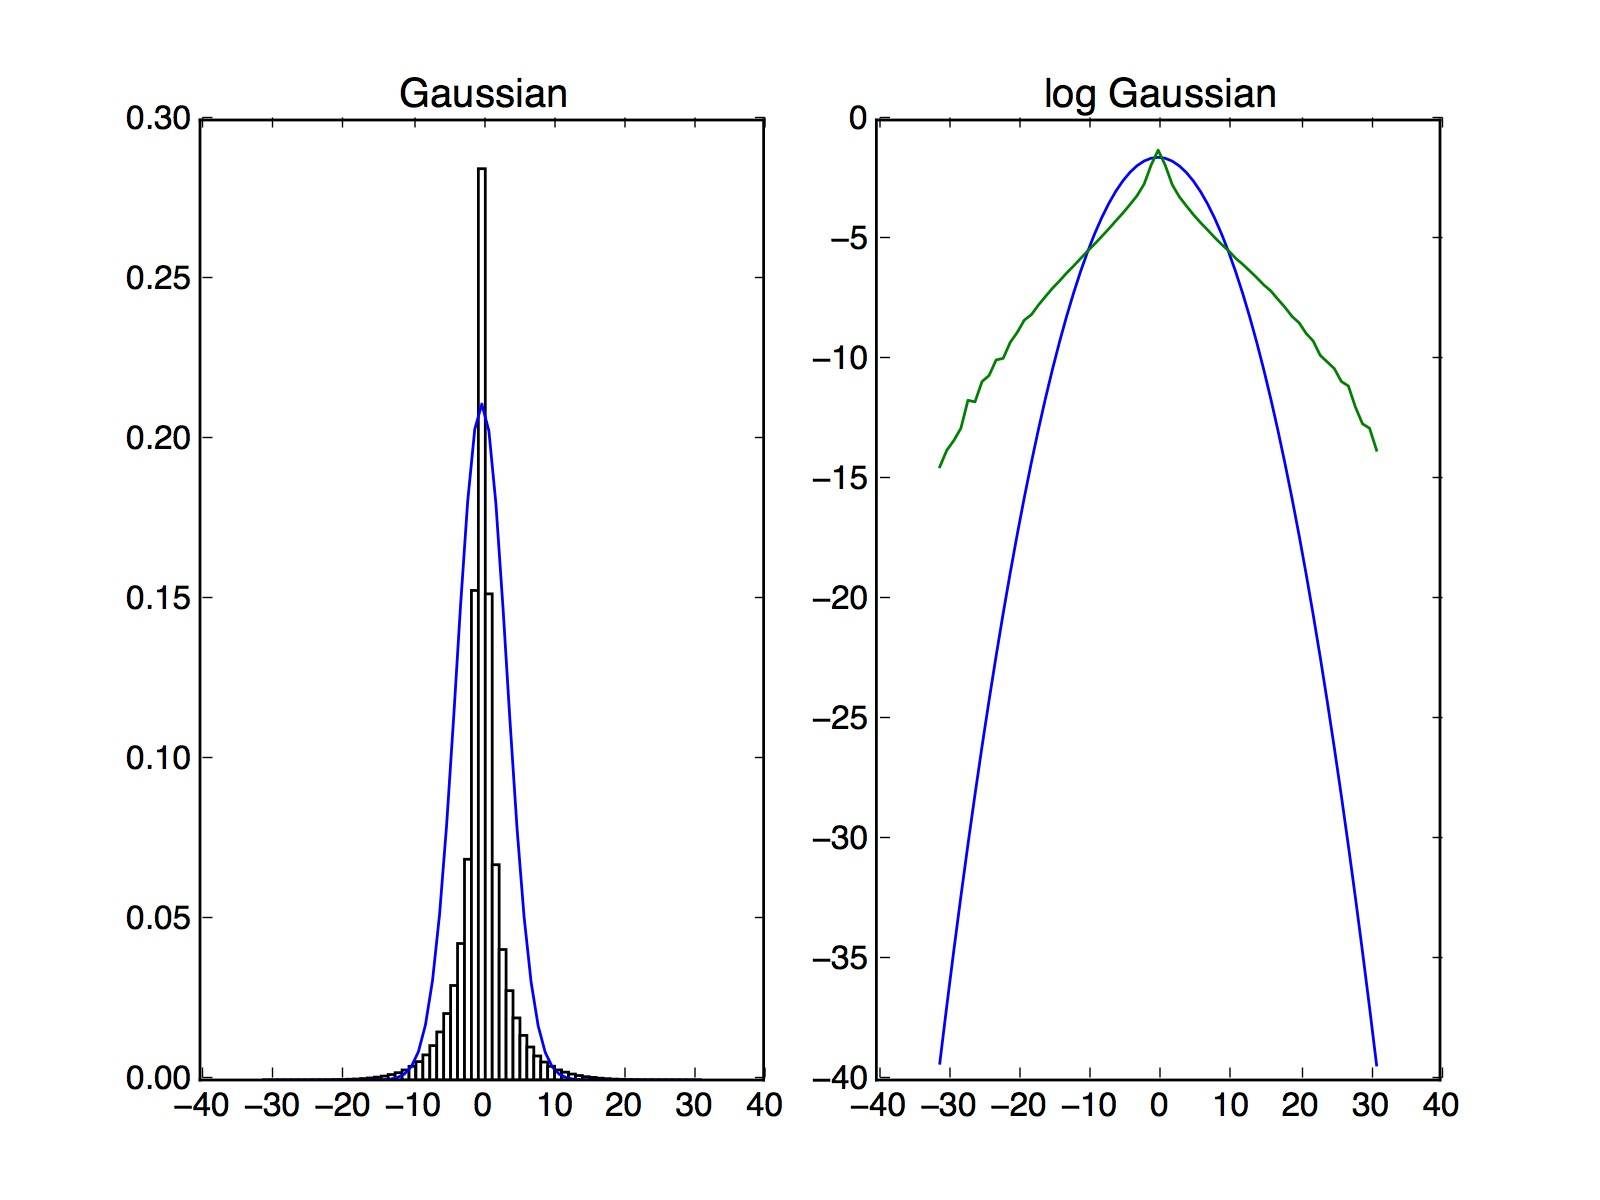
\includegraphics[height=10cm]{results/q1_4.jpg}{\\figure 3 Gaussian fit}
\end{center}
Superimposing a Gaussian distribution on the histogram, we can see that the histogram is much more narrow, which confirms with our analysis in 1.4 that the pixels are not sampled randmly.\\
\item{1.5}
We then down sampled the image by 2x2 and 4x4 average, overlayed their histograms and obtain the following results.
\begin{center}
		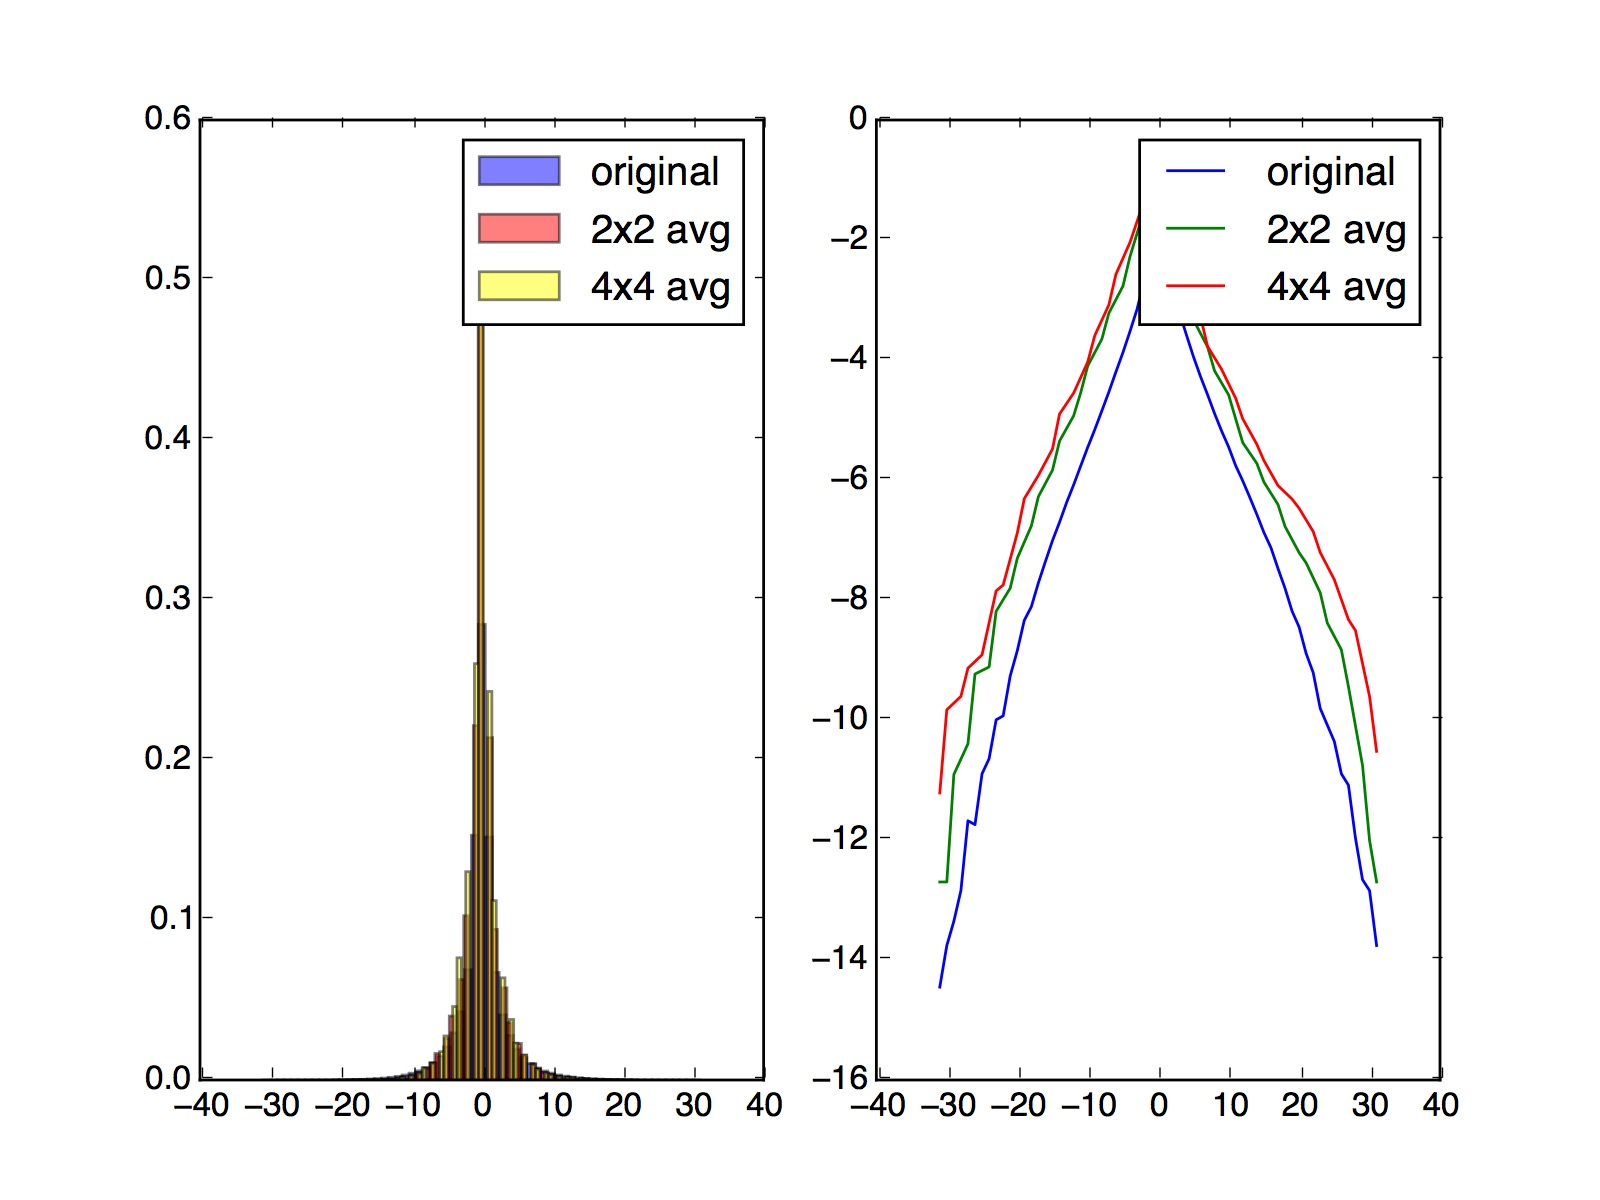
\includegraphics[height=10cm]{results/q1_5.jpg}{\\figure 4 histograms of down sampled images}
\end{center}
From the histograms we can see that they overlap very well, meaning the distribution is almost unchanged under different scale. This means that the structure of the data is maintained under down sampling. And it makes sense because after down sampling, we can still understand the scene in the image, and so the structure information should be maintaiend. The scale invariant phenomenon is actually an indicator that the dimensionality the content of the image should be much smaller than the image space itself.\\
\item{1.6}
To compare with the natural image, we syntheized a random noise image and repeated procedure 1-2-4, and obtaind the following results.
\begin{center}
		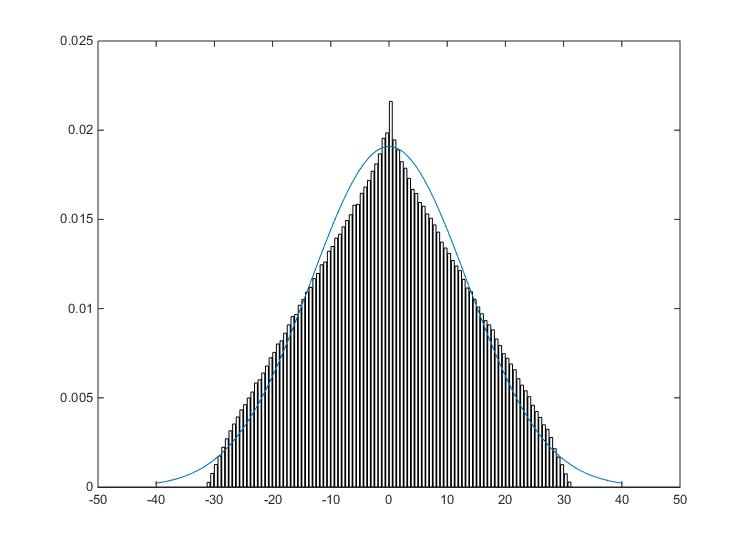
\includegraphics[width=8cm]{results/1_7_randm_superimpose.jpg}
		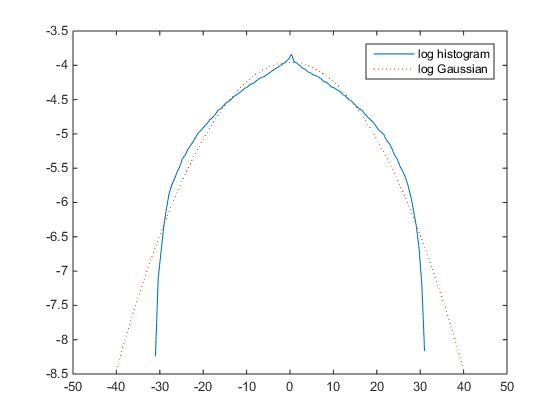
\includegraphics[width=8cm]{results/1_7_randm_superimpose_log.jpg}{\\figure 5 gaussian fit of random noise}
\end{center}
From figure 5 above we can see that the histogram fits its Gaussian distribution very well. This makes sense because with the random image, gradient filter generates sums of uniformly distributed pixel values, which yields a Gaussian distribution by the central limit theorem. And this differs from the histogram of structured data of a natural scene.\\
\end{problem}

\begin{problem}{2. Verify the 1/f Power Law in Natural Images}
\item{}
For this question we performed Fourier transform on several natural images and plotted the power sepctrum in order to verify the 1/f power law.\\
\item{2.1}
For four images of natural scenes, we performed fft2 with Matlab, and plotted log(A(f)) against f, where is the norm of frequencies on each direction. Below are the results.
\begin{center}
		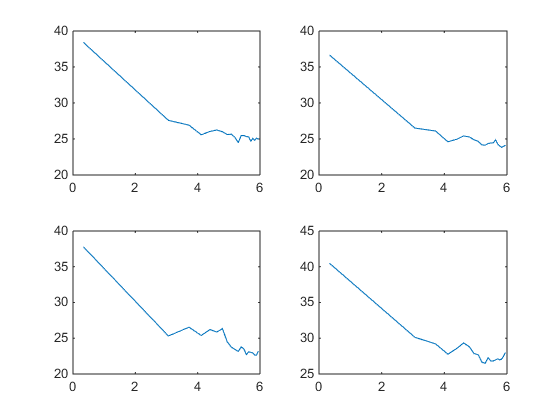
\includegraphics[width=14cm]{results/q2_1.png}{\\figure 7 log(f) against log(A(f))}
\end{center}
Altough with some fluctuations, we can see that $A(f) \propto -log(f)$, which confirms the 1/f power law.
\begin{align*}
	A(f) \propto f
\end{align*}
\item{2.2}
Since $A(f) \propto f$, it is easy to show that
\begin{align*}
	S(f) = \int_{f}^{2f} A^2(x) dx \propto ln(2f) - ln(f) = ln2
\end{align*}
So plotting $S(f)$ against $f$ should give us an horizontal line. And it is confirmed by the observation below.
\begin{center}
		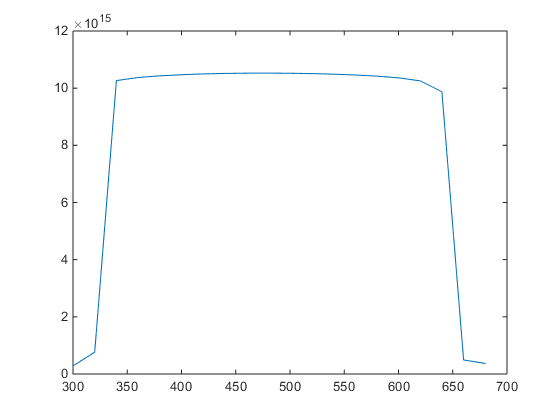
\includegraphics[width=10cm]{results/q2_2.png}{\\figure 8 $A^2(f)$ against f}
\end{center}
\end{problem}

\begin{problem}{3. A 2D Scale Invariant World}
\item{}
For this question we sampled images of random lines of length $p(r) \propto 1/r^3$ at different scales. And we croped 128x128 windows on them to observe the scale invariant nature of these images.\\
\item{3.1 3.2 Simulating images of random lines at different scale\\}
To simulate random lines, we represent each line with four parameters $(x, y, \theta, r)$, where $x, y$ represents its "starting point" in a 2D world, $\theta$ represent its direction, and $r$ represents its length. So both $x, y$ and $\theta$ can be drawed from a random number generator of uniform distribution. But since $\int_{0}^{\infty} 1/r^3 = \infty$, we added an offset and defined the distribution of length as
\begin{align*}
	p(r) = \frac{1}{2}\frac{1}{(r+0.5)^3} \ ,\ r \in [0, \infty)
\end{align*}
Thus the CDF is
\begin{align*}
	Pr(r) = \int_{0}^{r} p(r)dr = -\frac{1}{(2r+1)^2} + 1
\end{align*}
Therefore we can sample the length from a uniform random variable using the inverse of the CDF
\begin{align*}
	r = -\frac{1}{2} - \frac{\sqrt{1-x}}{2(x-1)}
\end{align*}
Picking N = 4000, we were able to generate images of random lines of 1024x1024 like below. To down sample it into 512x512 and 256x256, we can simply resample it by setting $r' = r/2$, $r' = r/4$, respectively, and removing lines whos length below a threshold, for example 1 in our case.\\
\begin{center}
		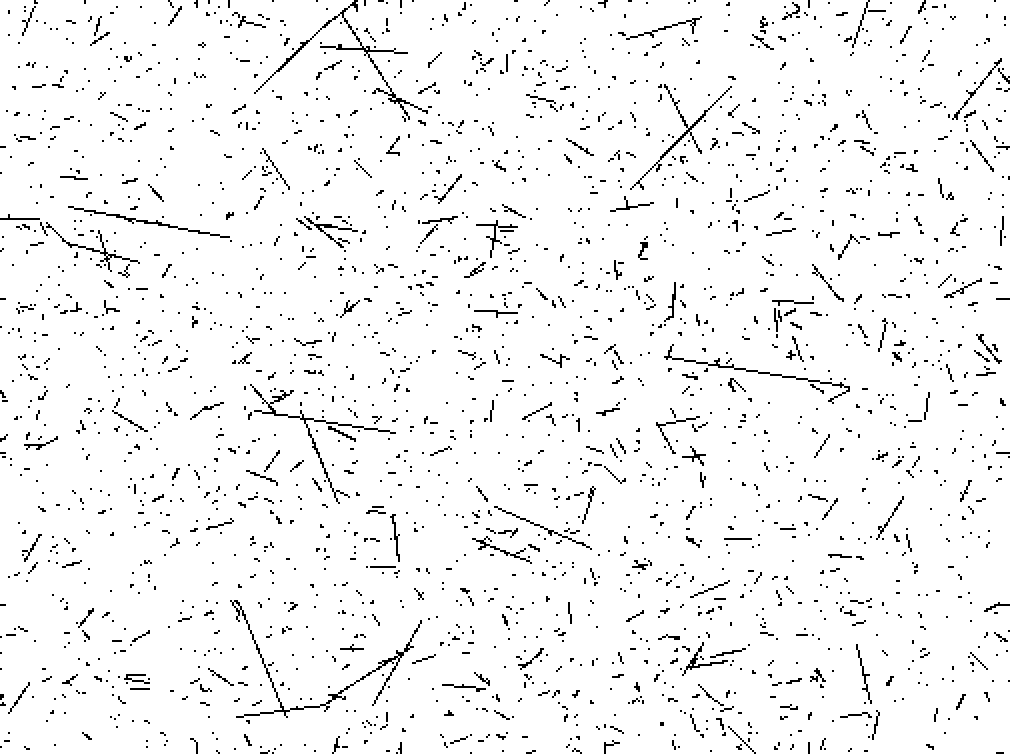
\includegraphics[width=8cm]{results/rand_lines.png}{\\figure 6 random lines}
\end{center}
\item{3.3}
Croping two 128x128 window from each image, we have the following 6 images.
\begin{center}
		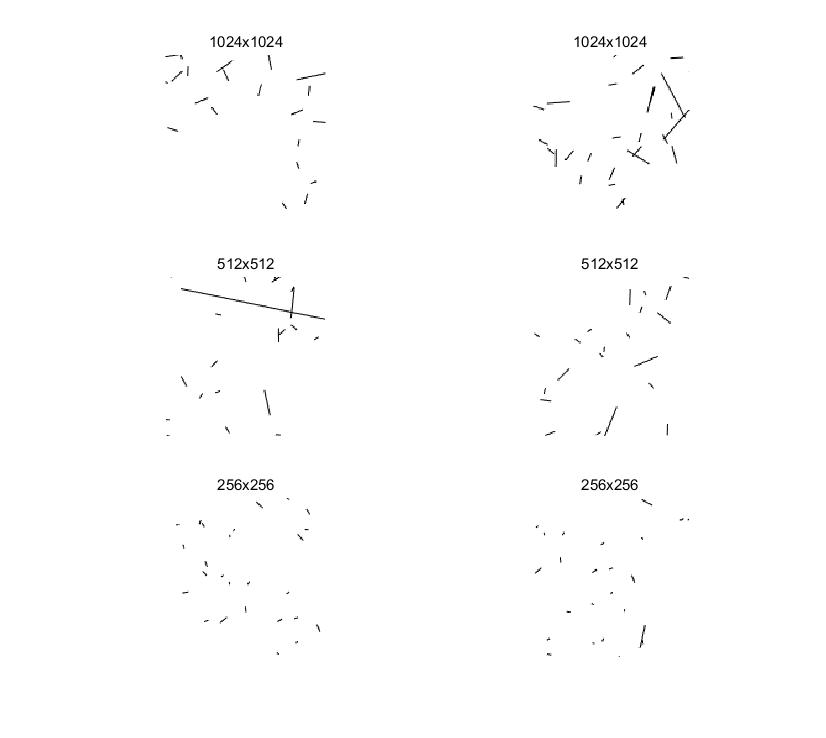
\includegraphics[width=18cm]{results/q4.jpg}{\\figure 7 128x128 window from different scales}
\end{center}
We can see that the windows from different scales looks very similar. This is due to the fact that the lengths we sampled decrease at $O(n^2)$ according to the CDF, which is the same as rate as the we down sample an image. Note that we choosed not to display a line if its length becomes too small, and if the display length threshold is not tuned properly, the down sampled images may have lots of small dots that are not present in larger sizes.

\end{problem}

% --------------------------------------------------------------
%     You don't have to mess with anything below this line.
% --------------------------------------------------------------
 
\end{document}
